\documentclass[11pt]{article}
\usepackage{graphics,epsfig,amsmath,amssymb}
\usepackage{epsf}
\usepackage{boxedminipage}
\usepackage{fullpage}
\usepackage{fancyheadings}
\usepackage{times}
\usepackage{amsmath}
\usepackage{ifthen}
%\usepackage{pseudocode}
\usepackage{psfrag}
\usepackage{url}
\pagestyle{fancy}

\setlength{\topmargin}{.2in}
\setlength{\parindent}{0in}
\setlength{\parskip}{.15in}
\setlength{\footskip}{0.1in}

\newcounter{pctr}
\stepcounter{pctr}

\newcounter{partctr}

\newcommand{\ie}{{\em i.e.}}
\newcommand{\eg}{{\em e.g.}}

\newcommand{\ch}{\item {\bf True~~/~~False~~}}
\newcommand{\tfnote}{\probnote{Circle True or False for each choice.}}
\newcommand{\allapply}{\probnote{Circle ALL that apply}}
\newcommand{\bestanswer}{\probnote{Circle the BEST answer}}
\newcommand{\ansbelow}{\probnote{Answer legibly in the space below.}}

\renewcommand{\thesection}{{\bf\Roman{section}}}
\renewcommand{\theenumi}{{\bf\Alph{enumi}.}}
\renewcommand{\labelenumi}{{\bf\Alph{enumi}.}}

\newcommand{\setversion}[1]{\def\version{#1}}
%\setversion{answers}
\setversion{quiz}

\ifthenelse{\equal{\version}{answers}}{
    \newcommand{\sols}[1]{#1}
}{
    \newcommand{\sols}[1]{}
}


\begin{document}

\newcounter{answer}
\newenvironment{answer}[1][\relax]{\refstepcounter{answer}\begin{list}%
 {}{\leftmargin 0pt\rightmargin 0pt\labelsep 3pt\parsep 0pt%
 \setlength{\listparindent}{\parindent}}
    \item {\bf Answer \theanswer #1}\
    }{\hspace*{\fill}$\blacksquare$\end{list}} 



% uses these macros to delimit problems
\newcommand\prob[1]%
  {\begin{itemize}\item[]%
   \vspace{.2in}{\bf\thepctr. ~[#1~ points]:}\stepcounter{pctr}}
\newcommand\eprob{\end{itemize}}
\newcommand\probnote[1]%
  {\\\begin{tabular}{cr} \hspace{3in} & {\bf (#1)} \\ \end{tabular}}

% headers/footers
\lhead[\fancyplain{}{\bf Page \thepage ~of \pageref{lastpage}}]%
      {CS 6250 Spring 2014, Quiz 2}
\lfoot[{\bf Name: }]%
      {{\bf Name: }}
\rhead[CS 6250 Spring 2014, Quiz 2]%
      {\fancyplain{}{\bf Page \thepage ~of \pageref{lastpage}}}
\cfoot{}
%\setlength{\headrulewidth}{0in}
\setlength{\headsep}{.3in}

 % Compact itemize and enumerate.  Note that they use the same counters and
% symbols as the usual itemize and enumerate environments.
\def\compactify{\itemsep=0pt \topsep=0pt \partopsep=0pt \parsep=0pt}
\let\latexusecounter=\usecounter
\newenvironment{CompactItemize}
  {\def\usecounter{\compactify\latexusecounter}
   \begin{itemize}}
  {\end{itemize}\let\usecounter=\latexusecounter}
\newenvironment{CompactEnumerate}
  {\def\usecounter{\compactify\latexusecounter}
   \begin{enumerate}}
  {\end{enumerate}\let\usecounter=\latexusecounter}


\cfoot{}
\pagestyle{empty}

\begin{center}
\begin{tabular}{lr}
\resizebox{1in}{!}{\includegraphics{GT}}
&
\parbox{4in}{
    {\Large\it College of Computing} \\ \\
    {\LARGE\sf Georgia Institute of Technology} 
}
%
\end{tabular}
\end{center}

\begin{center}
{\Large{\bf CS 6250: Computer Networking: Spring 2014} \\
 \vspace{.15in} \Huge{\bf Quiz II}} 
%\vspace{.2in}

% this is the box on the first page with overall quiz information
\begin{boxedminipage}[h]{6in}
There are \underline{14 questions} and \underline{\pageref{lastpage}
  pages} in this quiz booklet (including this page).  Answer each
question according to the instructions given.  You have {\bf 85
  minutes}.

%\vspace{.1in} The last page is an easy question.  {\em Rip this
%page off of your exam for five bonus points.}  Turn it in anonymously if
%you like.


\vspace{.1in} 
If you find a question ambiguous, write down any
assumptions you make.  {\bf Be neat and legible.}  If I can't
understand your answer, I can't give you credit!  You may want to look
through the whole quiz to identify which questions you can complete most
quickly for the most points.

\vspace{.1in} 
Use the empty sides of this booklet if you need scratch space.  You
may also use them for answers, although you shouldn't need to.  {\em If you
do use the blank sides for answers, make sure to clearly say so!}

\vspace{.1in} 
{\bf Note well: Write your name in the space below AND your initials at the bottom of each
page of this booklet.}

\begin{center}{\bf THIS IS AN ``CLOSED BOOK'' QUIZ.\\
YOU ARE PERMITTED ONE DOUBLE-SIDED SHEET OF PAPER FOR NOTES.\\
{\em ABSOLUTELY NO EMAIL OR MESSAGING OF ANY KIND!} \\
MAKE SURE YOU'VE READ ALL THE INSTRUCTIONS ABOVE!}
\end{center}
{\em Initial here to indicate that (1)~you've read the instructions and (2)~
you agree to abide by the Georgia Tech Honor Code: }

\vspace{.1in} The last page has easy bonus questions, which you can
answer outside of the allotted time.  Rip the last page off of your
quiz for five bonus points.  Turn it in anonymously if you like.

\end{boxedminipage}
\end{center}
\vspace*{0.25in}
\begin{center}
{\it Do not write in the boxes below}
\end{center}

\begin{center}
\begin{tabular}{|l|l|l|l|l|l|l|l|l|} \hline \hline
{\bf 1-5 (xx/20)}& {\bf 6-9 (xx/20)}& {\bf 10-12 (xx/30)} & {\bf 13-14 (xx/30)} & {\bf Total
  (xx/100)}  \\ \hline 
 & & & & \\ 
 & & & &\\ \hline \hline
\end{tabular}
\end{center}

\vspace{.2in}
{\bf\Large{Name:}}

\newpage
\pagestyle{fancy}

\section{Warmup}

\prob{4} What are some of the possible causes of congestion collapse?
\allapply

\setcounter{partctr}{0}
\begin{list}{\bf\Alph{partctr}.}{\usecounter{partctr}}
\item Faulty router software
\item Spurious retransmissions in flight
\item Packets traveling distances that are too far in between routers
\item Undelivered packets
\item None of the above.
\end{list}
\eprob

\sols{
\begin{answer}
The answer is: (B), (D).
\end{answer}
}


\prob{4} Which of the following are true about additive increase
multiplicative decrease (AIMD) and fairness?
\allapply
\setcounter{partctr}{0}
\begin{list}{\bf\Alph{partctr}.}{\usecounter{partctr}}
%\begin{enumerate}
\item Additive increase improves efficiency.
\item Additive increase improves fairness.
\item Multiplicative decrease improves efficiency.
\item Multiplicative increase improves fairness.
\item All of the above.
\end{list}
\eprob

\sols{
\begin{answer}
The answer is: (A), (D).
\end{answer}
}

\prob{4} Which of the following pathologies can streaming audio and
video tolerate by adding more buffering at the receiver?
\allapply
\setcounter{partctr}{0}
\begin{list}{\bf\Alph{partctr}.}{\usecounter{partctr}}
%\begin{enumerate}
\item Packet loss
\item Delay variation or jitter
\item Low throughput
\item Out of order packets
\item All of the above
\end{list}
\eprob

\sols{
\begin{answer}
The answer is (A), (B), (D).
\end{answer}
}

\newpage
\prob{4} 
Which of the following statistics are possible to gather from
information such as flow sampling (\eg, NetFlow)?
\allapply
\setcounter{partctr}{0}
\begin{list}{\bf\Alph{partctr}.}{\usecounter{partctr}}
%\begin{enumerate}
\item The time in between each packet transmission
\item Packet headers
\item The number of bytes that each flow sends
\item The number of packets that each flow sends
\item None of the above
\end{list}
\eprob

\sols{
\begin{answer}
The answer is: (C), (D).
\end{answer}
}


\prob{4}  Which of the following are true about a leaky bucket traffic shaper?
\bestanswer
\setcounter{partctr}{0}
\begin{list}{\bf\Alph{partctr}.}{\usecounter{partctr}}
%\begin{enumerate}
\item A link that is shaped with a leaky bucket traffic shaper will
  never send traffic on the outgoing link at a rate that is higher than
  the average drain rate of the bucket.
\item On a link that is shaped by a leaky bucket, a sender can never
  send traffic faster than the average drain rate of the bucket; the
  link will simply drop any traffic that is sent at a higher rate.
\item Comcast's PowerBoost is likely implemented with a leaky bucket
  traffic shaper.
\item None of the above
\end{list}
\eprob

\sols{
\begin{answer}
The answer is: (A).
\end{answer}
}




\newpage
\section{Potpourri}

\prob{5} Suppose the round trip time between the sender and receiver is
100~milliseconds and the window size is 20 packets, and each packet is
1500 bytes. What is the rate at which the sender is sending? Please put
your answer here in terms of kilobits per second, keeping in mind that 1
byte is 8 bits.  (You can use 1000 bytes for 1~KB, to keep your math
simple.) ~\ansbelow 
\vspace*{2.5in}
\eprob


\prob{5} Suppose that the sustained rate that a subscriber subscribes to
is 10 megabits per second, but they would like to ``burst'' at a rate of
fifteen megabits per second. Suppose that the bucket size is one
megabyte, or 8~megabits. How long can the sender send at the higher
rate? Please give your answer in decimal form in seconds.  ~\ansbelow
\vspace*{1.5in}
\eprob

\newpage
\prob{5} What are two reasons why measuring TCP throughput {\em from a home
router} (as opposed to from a laptop on the same network connected via
the home wireless network) may provide a more accurate reading of the
TCP throughput of the access link?  ~\ansbelow
\vspace*{2.5in}
\eprob

\prob{5} Given a link of a certain bandwidth and packet loss rate,
explain why using multiple TCP connections in parallel can achieve
higher throughput than a single TCP connection.  ~\ansbelow
\vspace*{1.5in}
\eprob



\newpage
\section{Congestion Control and Streaming}

\prob{20} 
In this problem, you will derive the relationship between TCP
throughput, round-trip time, and packet loss.  We'll do the derivation
step-by-step. You won't need to know any calculus, but you'll need to
use the formula for computing the area of a triangle: $\frac{1}{2}\cdot
b\cdot h$. Consider the TCP window evolution shown in the diagram below
for your answers.  

\centering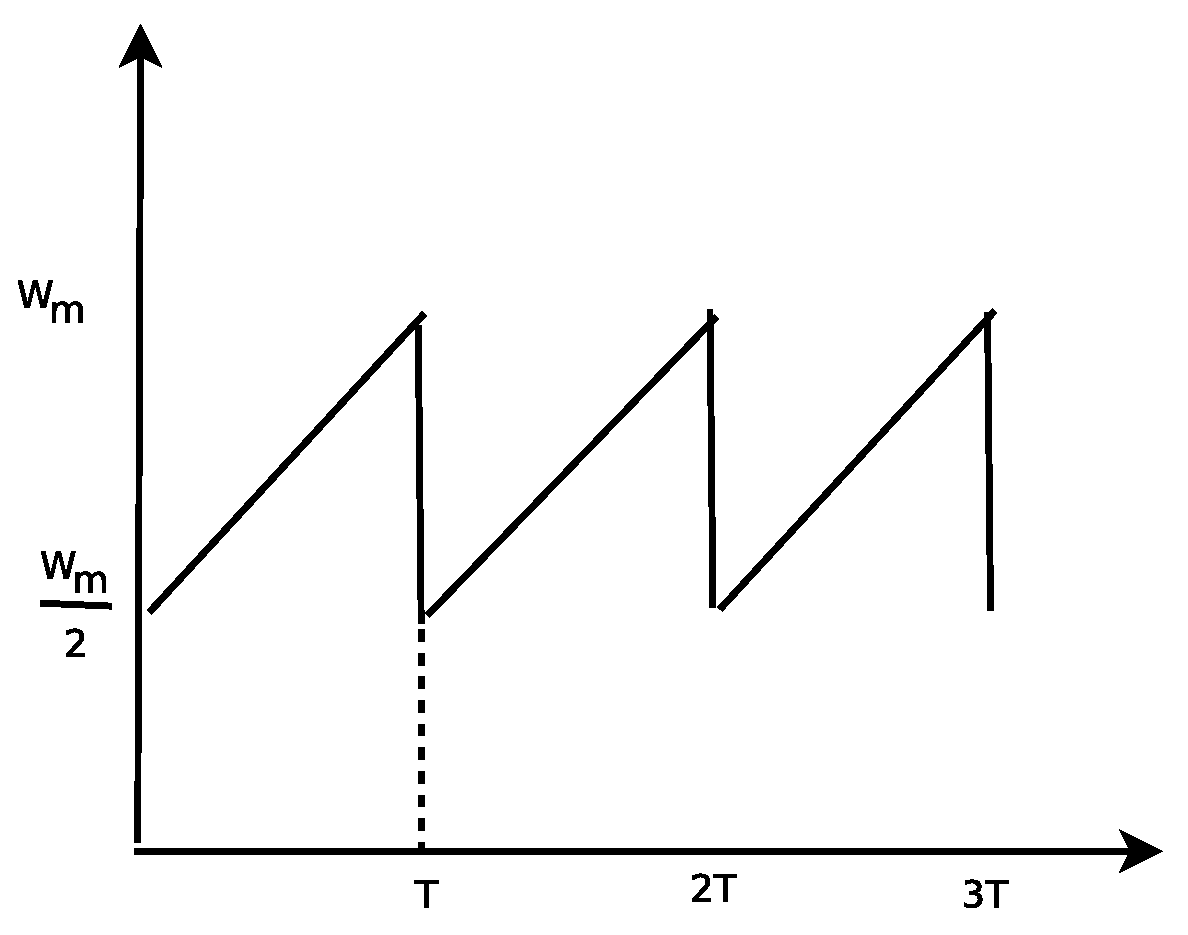
\includegraphics[width=0.5\linewidth]{tcp-window}

\begin{enumerate}
\item What is the number of packets in the TCP window right after a
  packet loss occurs?
\item What is the number of packets in the TCP window right before a
  packet loss occurs?
\item What is the total number of packets transmitted in between packet
  losses, in terms of $W_m$.  ({\em Hint:} Remember that, with additive
  increase, the TCP sender's window will increase by one packet per
  round trip. The formula for computing the area of a triangle may be
  useful in answering this question.).  {\em Your answer here is
    equivalent to $1/p$, where $p$ is the packet loss rate, and the
    number of bytes transmitted in between packet loss events is your
    answer here times the packet size $S$.}
\item How much time occurs between each packet loss, in terms of $W_m$
  and the round trip time $R$?
\item Express the TCP throughput, $\lambda$, in terms of your answers to
  the previous two questions.  Your answer should be in terms of $W_m$,
  $R$, and $S$.
\item Use the relationship between $p$ and $W_m$ from part (C) to
  substitute into your equation for $\lambda$ to obtain an equation for
  $\lambda$ in terms of $S$, $R$, and $p$.
\end{enumerate}


~\ansbelow\probnote{You can use the back of the page as well.}
\vspace{2in}
\eprob

\sols{
\vspace{-1in}
\begin{answer}
% http://blog.thousandeyes.com/a-very-simple-model-for-tcp-throughput/
\end{answer}
}

\newpage
\prob{5} George Burdell notes that as the throughput of a link
increases, the sender's TCP sending rate becomes more erratic, since the
difference between $W_m$ and $\frac{W_m}{2}$ becomes greater.  (This
problem of TCP on ``large bandwidth-delay product links'' is a
well-known phenomenon.)  For applications such as audio and video
streaming, George notes that this behavior could result in poor
performance. 

Explain why a large ``sawtooth'' the results from a high bandwidth link
could result in poor streaming performance.
 
~\ansbelow
\vspace{2in}
\eprob


\prob{5} George proposes two different ways of
mitigating the effects of TCP senders with large bandwidth-delay
products:
\begin{itemize}
\item Measuring the round-trip time and loss rate on a link from the
  sender and adjusting the throughput of the sender based on the TCP
  throughput equation (which you derived in the previous question).
\item Increasing the buffer size on bottleneck links so that packets can
  be transmitted from the buffer while the sending rate is below the
  average rate of the link.
\end{itemize}
Describe one advantage and one disadvantage of each approach, in terms
of either implementing the method described, or in terms of how well it
is likely to help the performance of a streaming application.
~\ansbelow
\vspace{2in}
\eprob

\sols{
\vspace{-1in}
\begin{answer}
% http://blog.thousandeyes.com/a-very-simple-model-for-tcp-throughput/
\end{answer}
}



\newpage
\section{Web Performance}

\prob{15} 
Consider the {\em partial} ``waterfall'' diagram shown below, which shows a Firefox client's
process of loading the home page at \url{http://gatech.com/}.

\centering\includegraphics[width=0.75\linewidth]{http-waterfall}

\begin{enumerate}
\item How many objects are being downloaded in parallel with the first
  object, the root document at \url{http://gatech.edu/} (the first row
  in the waterfall diagram?)
\item How many total DNS lookups are shown in the waterfall diagram?
\item Why is there not a DNS lookup for each object (\ie, why does each
  row in the waterfall diagram not show a TCP lookup)?
\item How many TCP connections appear to be operating in parallel to any
  single domain?  Justify your answer.
\item Why do rows 8--20 in the waterfall diagram not show TCP ``initial
  connections''? 
\end{enumerate}

~\ansbelow
\vspace{2in}
\eprob


\prob{15} 
The paper {\em Measuring and Mitigating Web Performance Bottlenecks in
  Broadband Access Networks} demonstrates that Web page load times stop
improving when the downstream throughput of the access link exceeds
about 16 Mbits/sec.  The paper claims that the latency of the connection
to the server becomes the primary bottleneck.

\begin{enumerate}
\item Give two steps in the process of retrieving a Web page where
  higher round-trip latency to the server can ultimately slow the
  overall page load time.
\item In class, we discussed how {\em increasing TCP's initial congestion
  window} could reduce the overall page load time.  Explain why.
\item We also discussed potential drawbacks of increasing TCP's initial
  congestion window.  List one drawback.
\item In class, we discussed how {\em prefetching certain parts of a Web
page load} could reduce the overall page load time.  Explain which
  aspects of a Web page load can be prefetched and how doing so can
  reduce page load time.
\item We also discussed potential drawbacks of prefetching.  List one drawback.

\end{enumerate}

~\ansbelow
\vspace{2in}
\eprob



\label{lastpage}
\end{document}
